% textidote: ignore begin
\subsection{Use Cases}\label{subsec:use-cases}
% textidote: ignore end
For a better understanding of how our solution will apply to the problem, we will in this section analyze
the use cases for the different action one can make in our solution.
% textidote: ignore begin
\begin{table}
    \centering
    \begin{tabularx}{0.7\textwidth}{ c X X X }
        \toprule
        \textbf{Use Case}& \textbf{Owner}& \textbf{Barista}& \textbf{Cognito}\\
        \midrule
        Login & \checkmark& \checkmark& \checkmark\\
        \midrule
        File uploading& \checkmark& \checkmark&\\
        \midrule
        Diagram viewing& \checkmark& \checkmark&\\
        \midrule
        Account handling& \checkmark&& \checkmark\\
        \bottomrule
    \end{tabularx}
    \caption{Use cases for Owner, Barista, and Cognito.}\label{tab:actors-tabel}
\end{table}
% textidote: ignore end
% textidote: ignore begin
\subsubsection{Login}\label{subsubsec:login_usecase}
% textidote: ignore end
Login is an active action from a barista or an owner, where they provide a username/mail and a password.
This action is then handled by Cognito, which verifies the credentials and responds with an error or a temporary token.
The token is then used as a prerequisite for other actions.

The Login action can be visualized through Figure~\ref{fig:cognito-conditional}
% textidote: ignore begin
\begin{figure}[H]
    \centering
    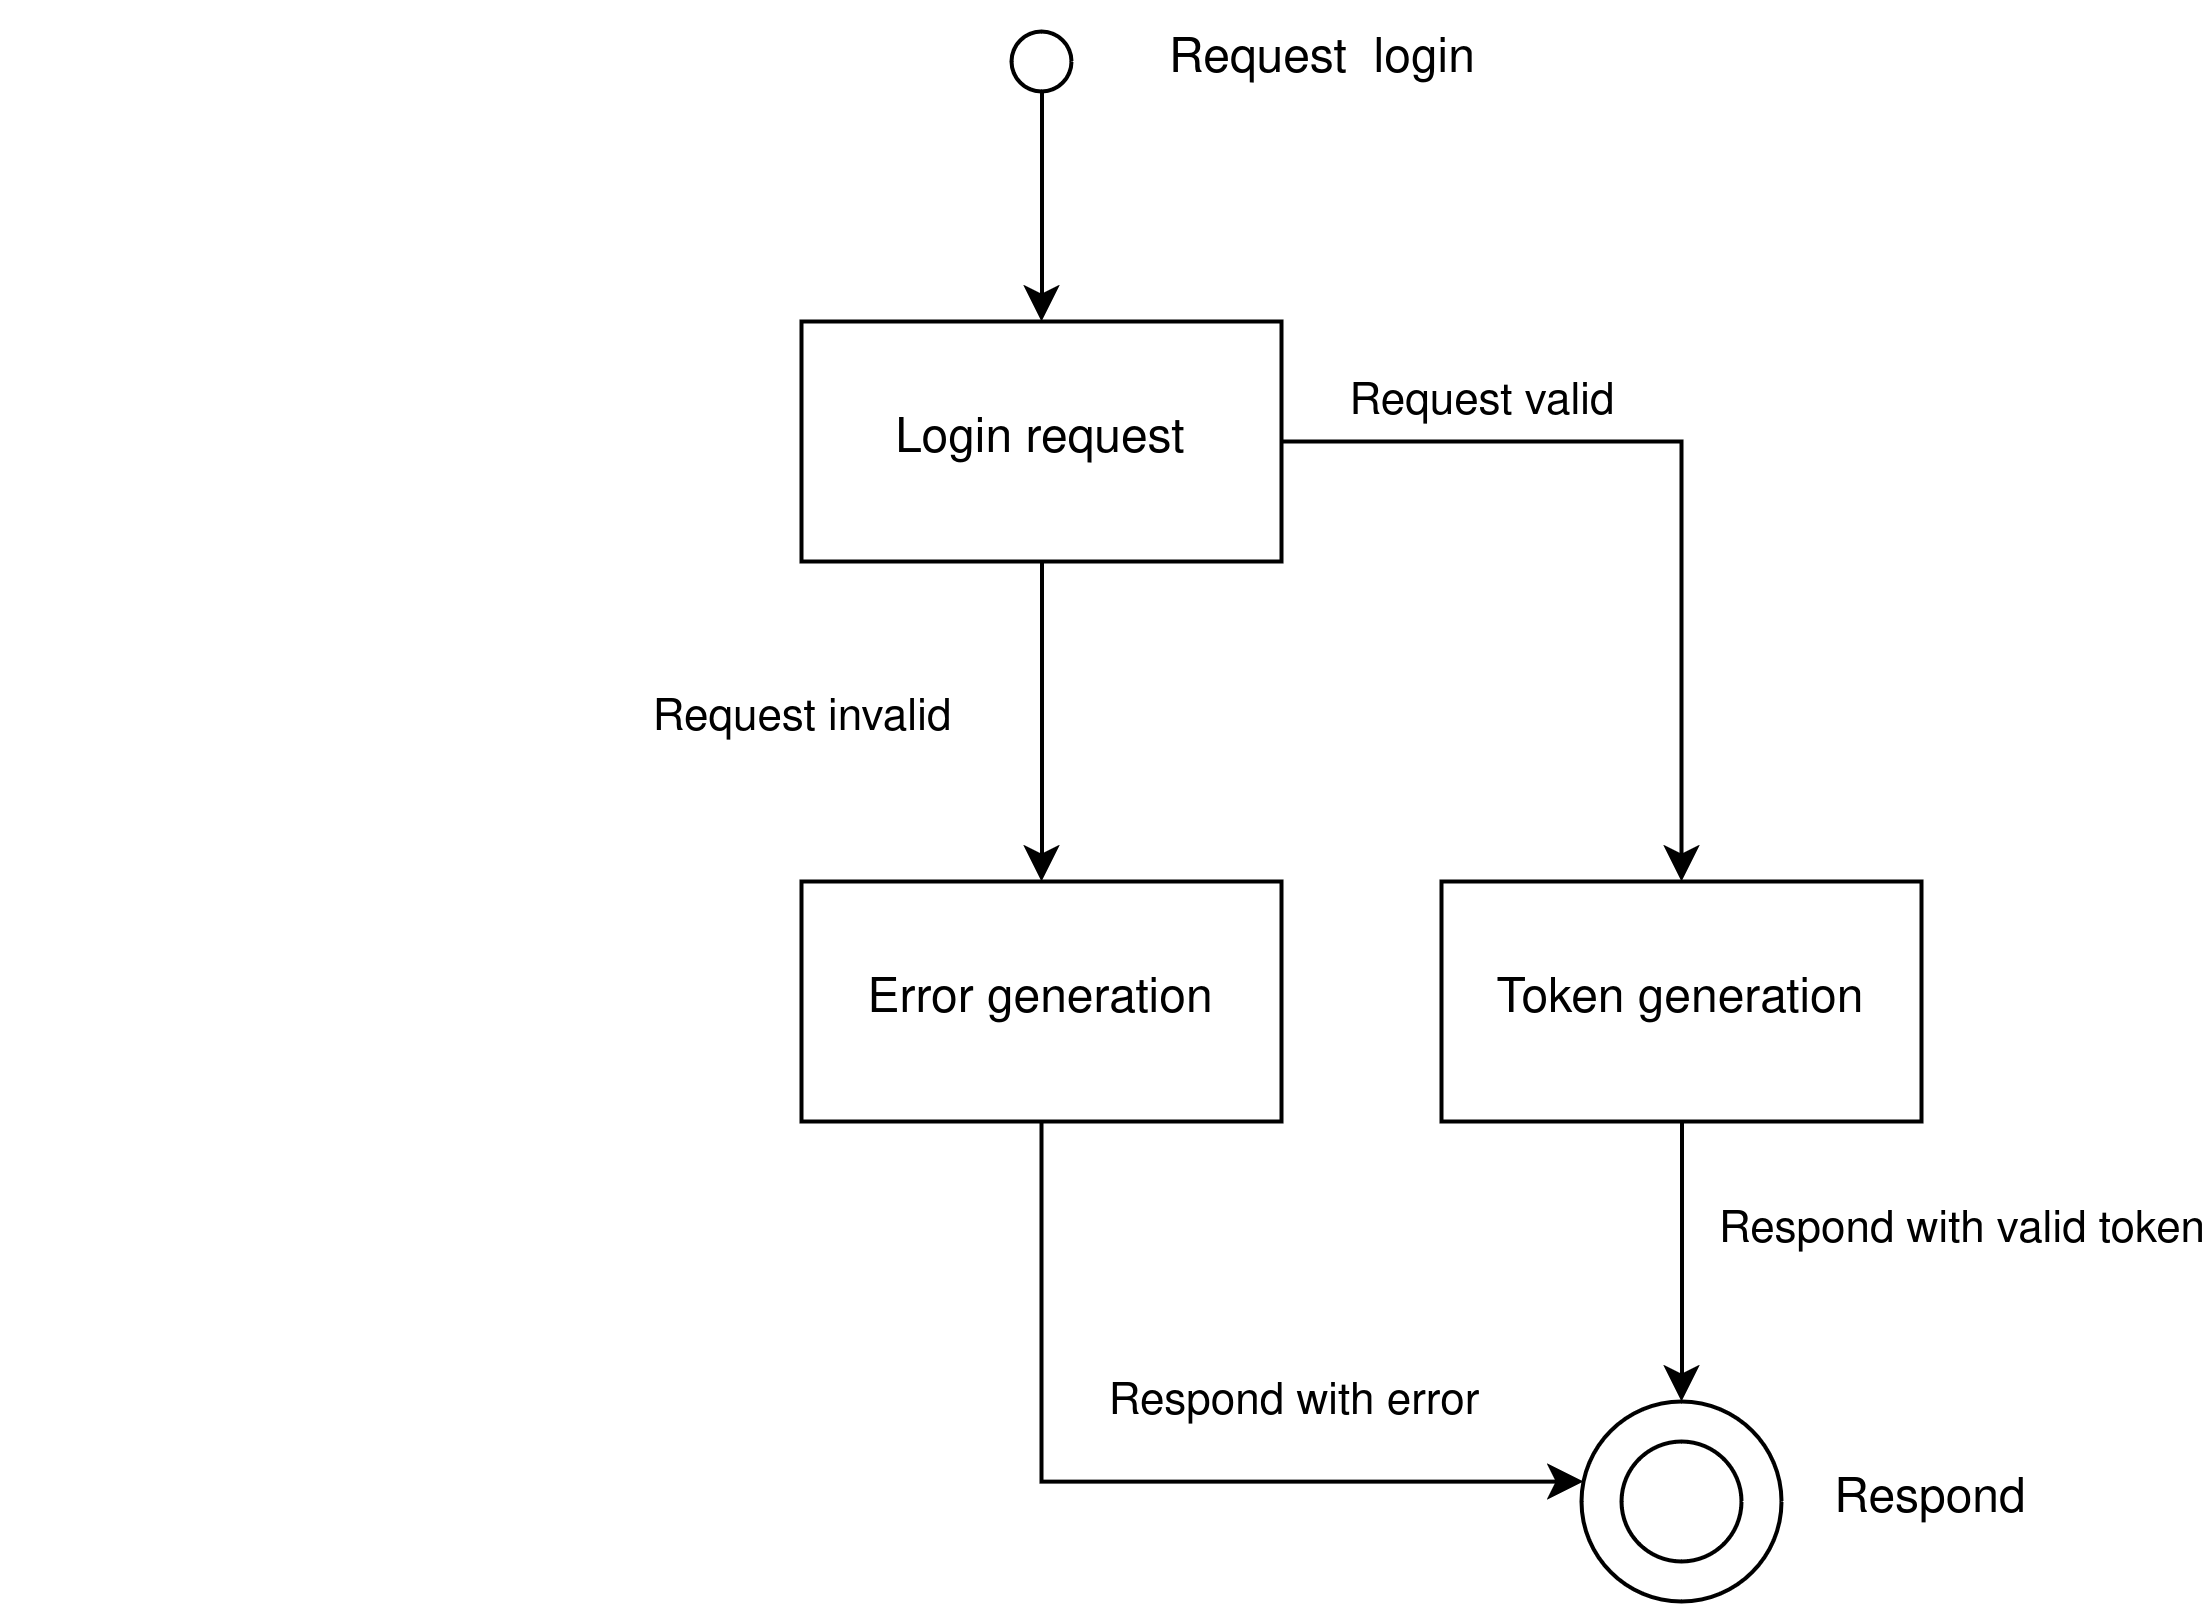
\includegraphics[width=0.6\textwidth]{ada-cognito}
    \caption{A diagram showing the Cognito actors use.}\label{fig:cognito-conditional}
\end{figure}

\subsubsection{File uploading}\label{subsubsec:file_uploading_usecase}
% textidote: ignore end
Uploading a file is an action actively made by either an owner or a barista.
The action will be triggered by clicking on an upload button on our webpage and selecting the appropriate file.
The server will then validate and parse the file which will result in a success or error,
which will be shown to the user.
We have shown how the workflow of uploading a file looks in both Figure~\ref{fig:barista-conditional},
and Figure~\ref{fig:owner-conditional}.

% textidote: ignore begin
\begin{figure}[H]
    \centering
    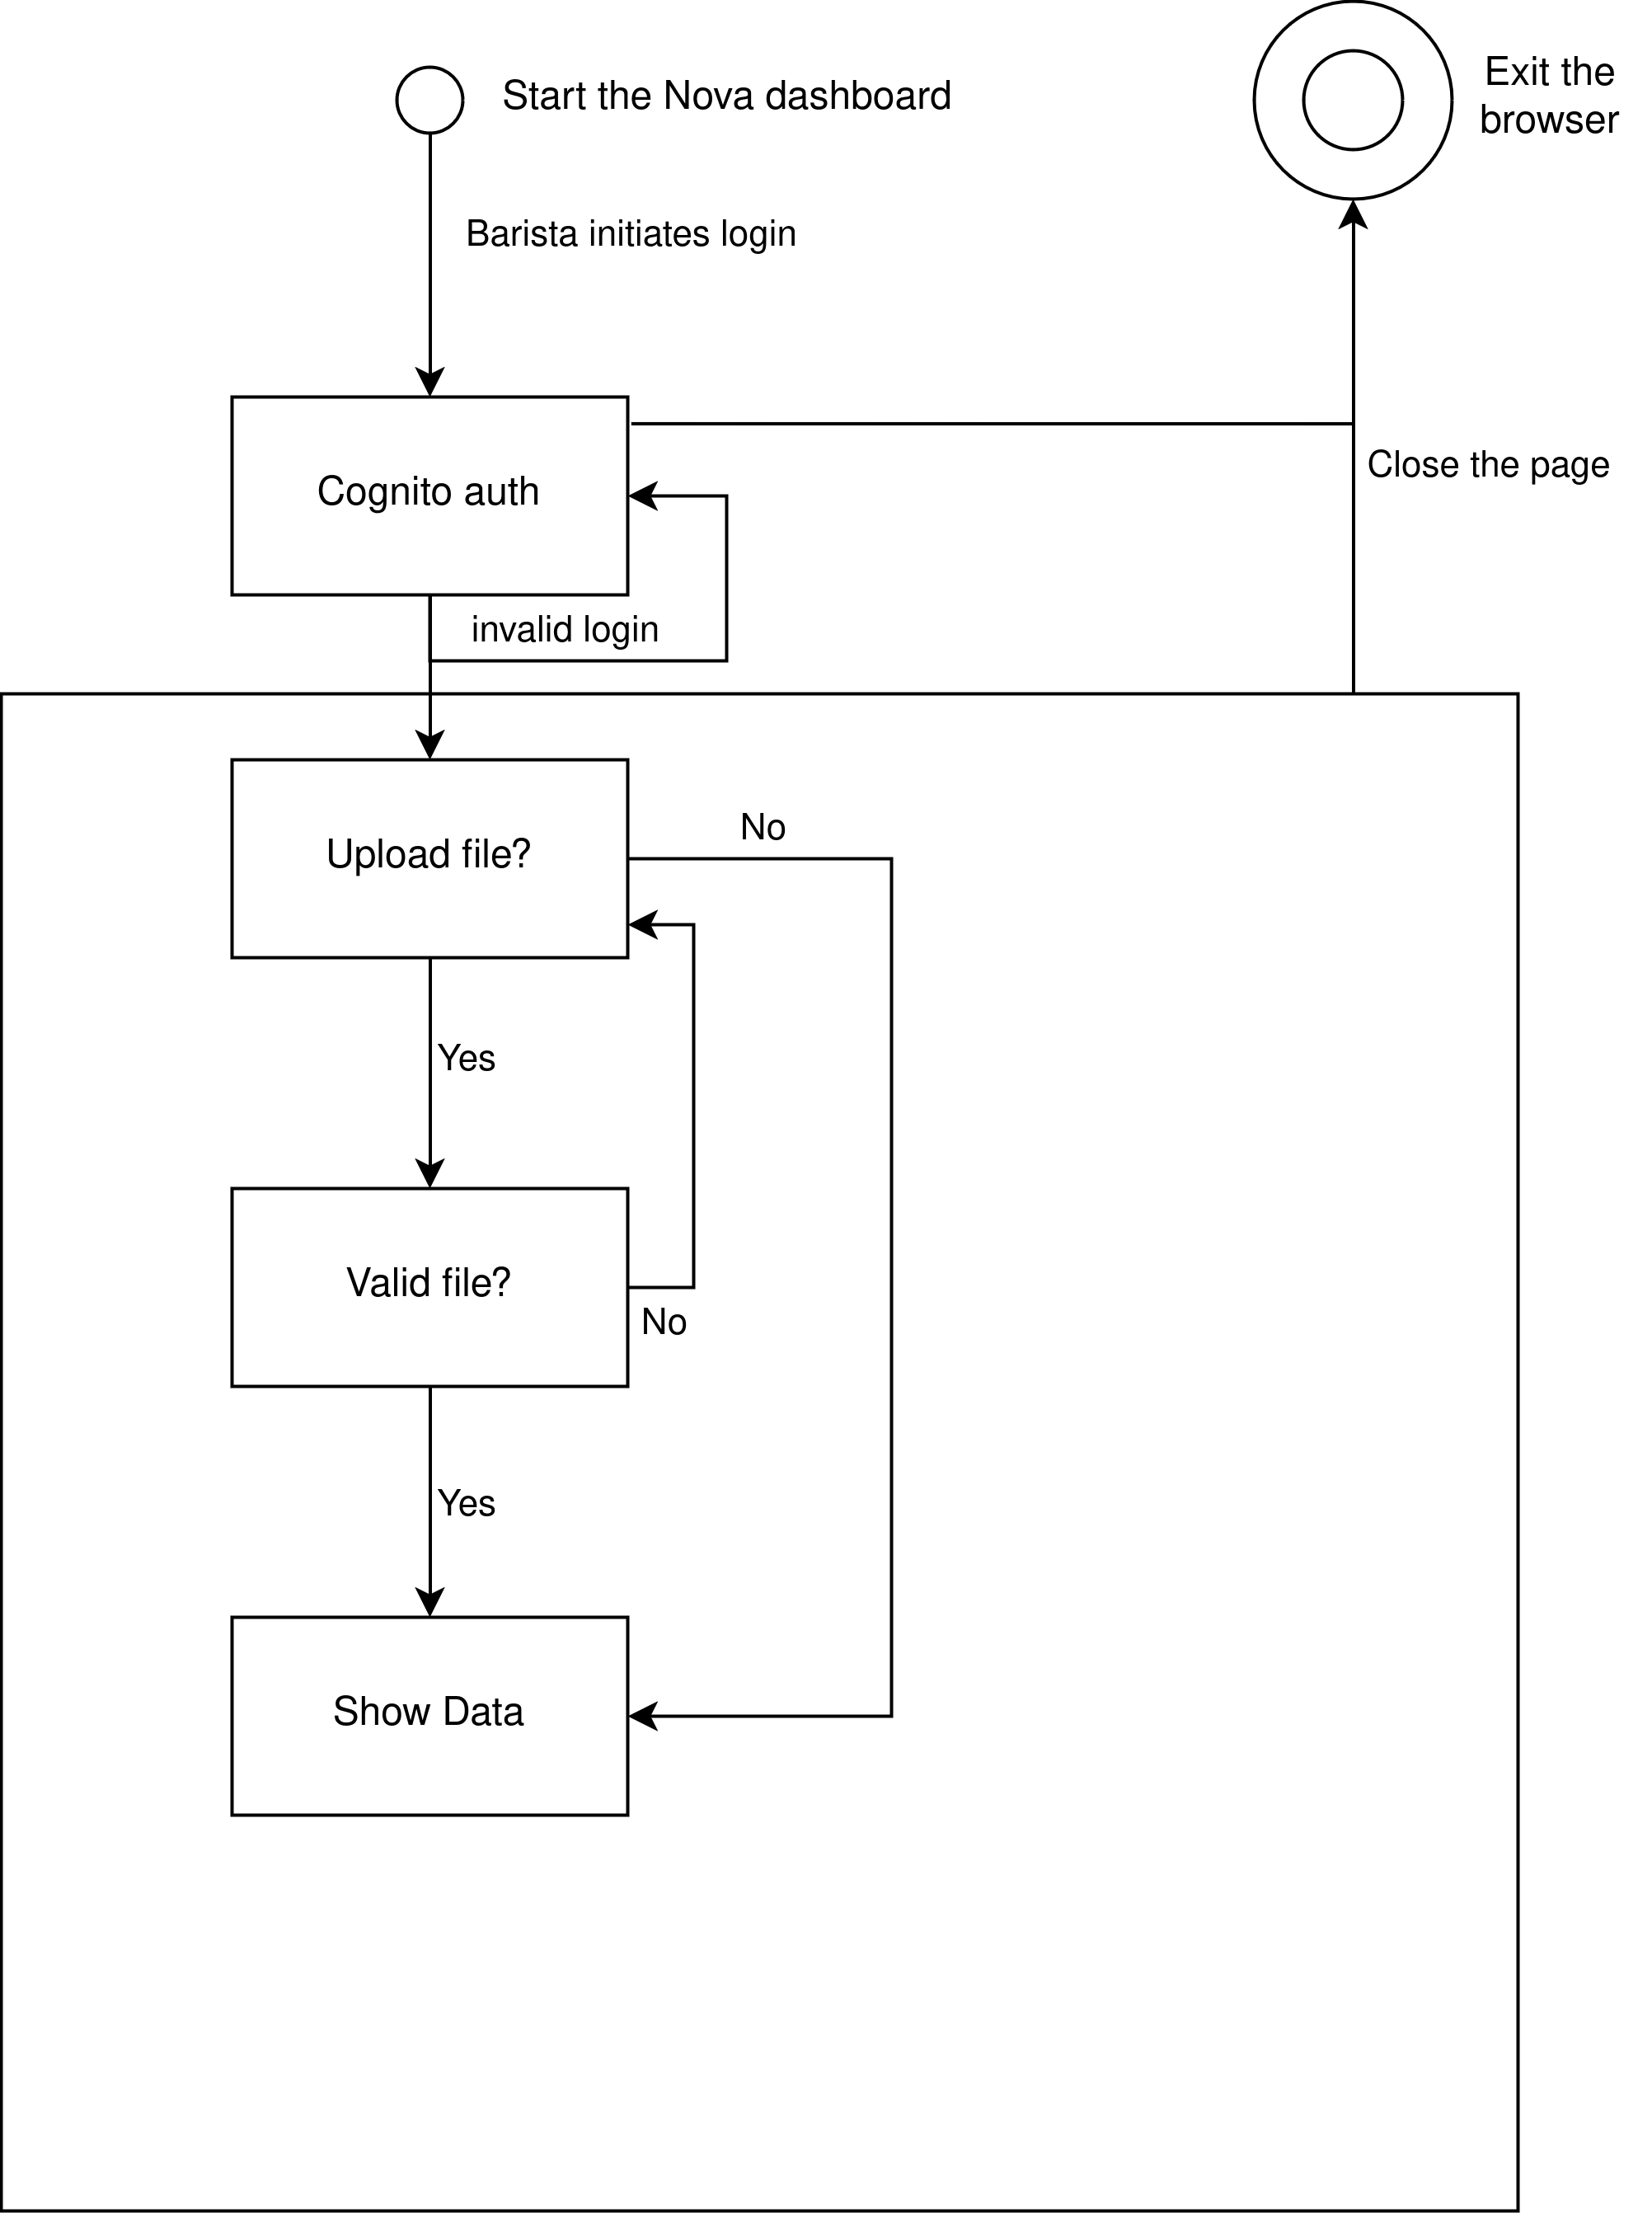
\includegraphics[width=0.6\textwidth]{ada-barista}
    \caption{A diagram showing a barista actors use.}\label{fig:barista-conditional}
\end{figure}

\subsubsection{Diagram viewing}\label{subsubsec:diagram_viewing_usecase}
% textidote: ignore end

After a successful login the user will immediately be directed to the dashboard that includes all diagrams.
Here the user can customize different aspects of the diagrams to get the easiest overview of their current problem.

% textidote: ignore begin
\subsubsection{Account handling}\label{subsubsec:account_handling_usecase}
% textidote: ignore end
Account handling is only possible for owners, the owners will then send an action to AWS Cognito, which will
do the actual creation, deletion or updating of users.
The use case for account handling can be seen in Figure~\ref{fig:owner-conditional}.

% textidote: ignore begin
\begin{figure}[H]
    \centering
    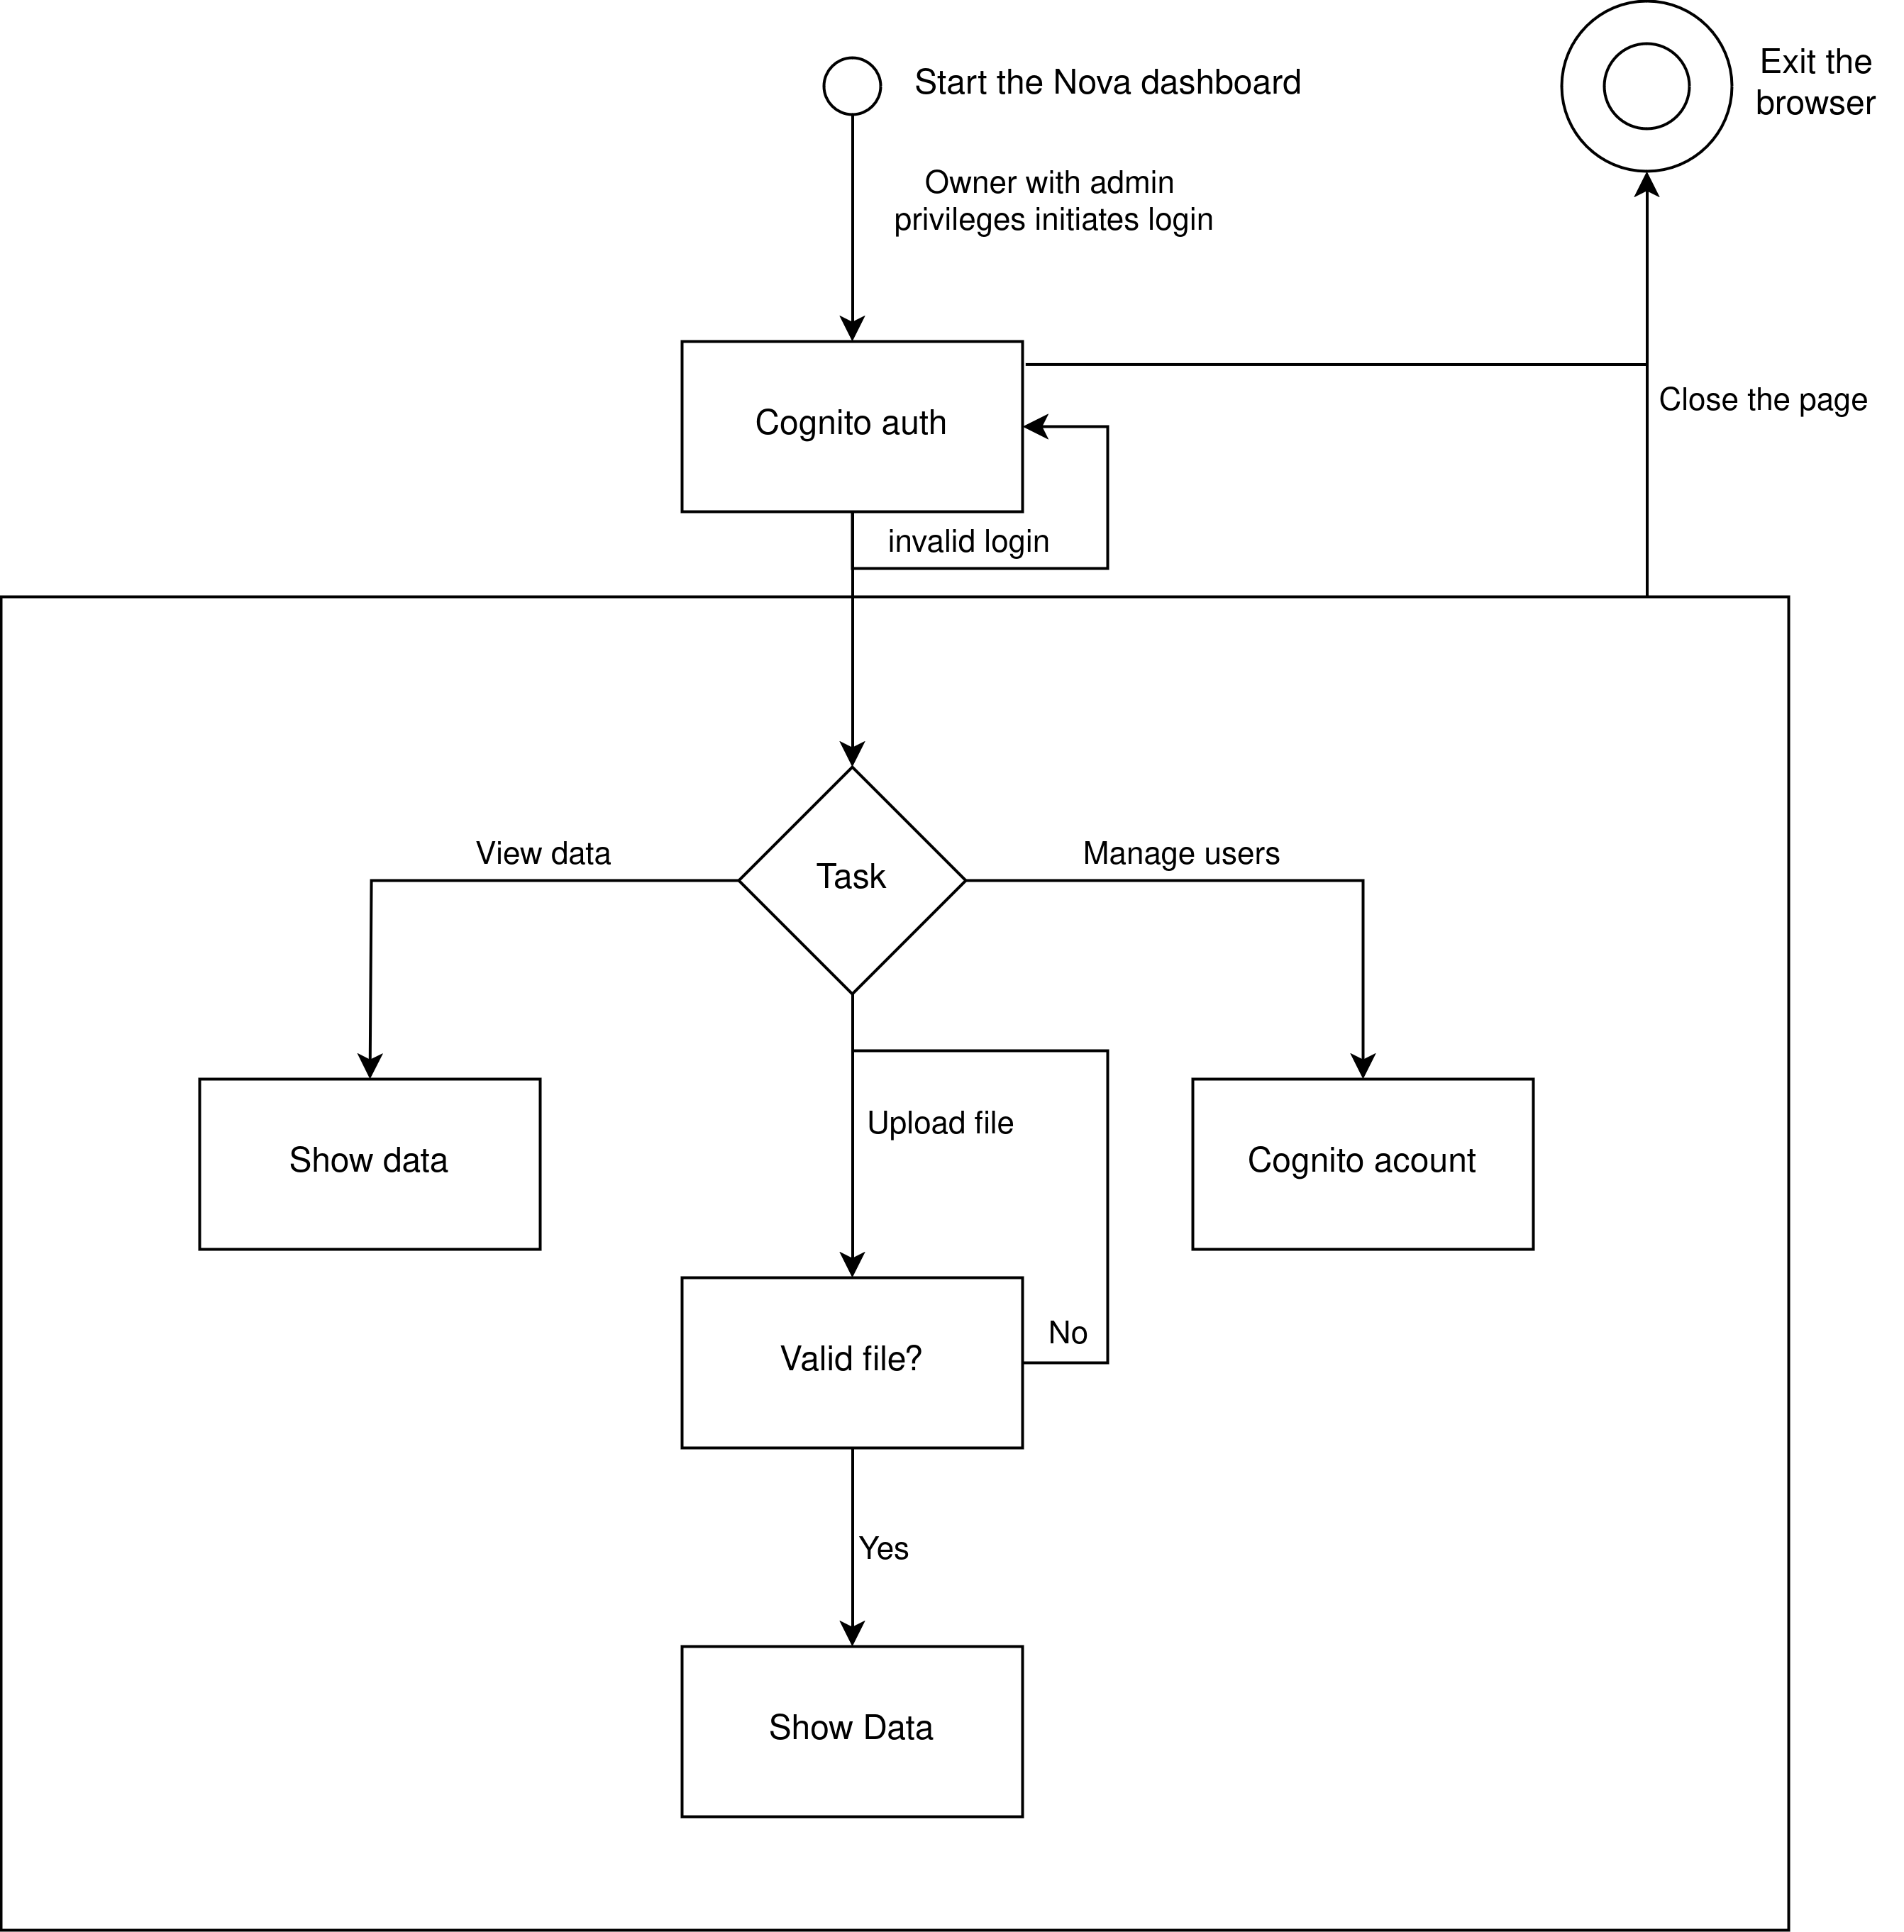
\includegraphics[width=0.6\textwidth]{ada-owner}
    \caption{Account handling A diagram showing an owner actors use.}\label{fig:owner-conditional}
\end{figure}
% textidote: ignore end